
\subsection{Регрессионный анализ}
\label{sec:experiment:regression}


В качестве первого способа анализа рынка недвижимости было решено использовать регресионный анализ.

В качестве инструмента для анализа данных было решено использовать язык программирования R. R — язык программирования
для статистической обработки данных и работы с графикой, а также свободная программная среда вычислений с открытым
исходным кодом в рамках проекта GNU. Язык создавался как аналогичный языку S, разработанному в Bell Labs, и является
его альтернативной реализацией, хотя между языками есть существенные отличия. Изначально R был разработан сотрудниками статистического факультета Оклендского университета
Россом Айхэкой (англ. Ross Ihaka) и Робертом Джентлменом (англ. Robert Gentleman)~\cite{r_lang}.

У R есть ряд преимуществ по сравнению с Python. Он интуитивно понятен, а потому удобен,
с точки зрения написания кода. Чтобы писать программы на R, необязательно соблюдать четкую структуру – можно просто
вводить последовательный набор команд, и этого будет вполне достаточно.

Язык R создавался специально для анализа данных, поэтому все конструкции синтаксиса достаточно емки и понятны.
Python — более универсальный и многоцелевой язык, что, естественно, усложняет его понимание.

Среди достоинств языка R можно отметить следующие:
\begin{itemize}
  \item Удобные и понятные языковые конструкции
  \item Базовые статистические методы реализованы в качестве стандартных функций, что значительно повышает скорость разработки.
  \item Есть несколько отличных пакетов для визуализации. Можно строить и двумерную графику (диаграммы, боксплоты), а также и трехмерные модели. Результаты проведенной работы часто становятся значительно понятнее и выразительнее.
  \item Для R разработано огромное количество дополнительных пакетов.
\end{itemize}

Распределение цены объекта недвижимости в зависимости от его площади показана на рисунке~\ref{fig:experiment:price_area_model}.
Можно заметить, что стоимость цены расчет с ростом площади, что ожидаемо, однако говорить о линейной зависимости не приходится.
Коэффициент детерминации $R^2$ равен 0.15, что является достаточно низким показателем и не позволяет говорить о сильной
взаимосвязи цены и площади.

\begin{figure}[!ht]
  \centering
  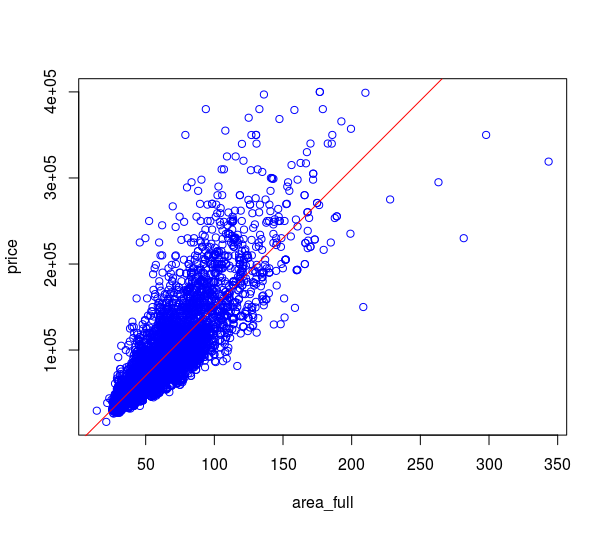
\includegraphics[scale=1]{price_area_model.png} 
  \caption{Зависимость цены от площади}
  \label{fig:experiment:price_area_model}
\end{figure}

Построим множественную модель регресии с учетом всех приведенных выше параметров. Анализ модели показан на
рисунке.

Данные характеристики показывают нам, что такие параметры как 
общая площадь, количество гаражей, количество открытых парковочных мест, тип объекта недвижимости, количество душевых комнат и спален,
средняя цены аренды недвижимости в районе являются значимыми и оказывают существенное влияние на формирование
окончательной цены. Количество парковочных мест под навесом, средняя цены аренды недвижимости в районе,
а также процент изменения арендной ставки не влияют на процесс формирования цены. Поэтому их можно исключить из модели.

Полученный коэффициент детерминации $R^2$ равен 0.48 оказался выше чем в модели парной регресии, однако он все еще
недосточно велик чтобы точно формировать цену на объекты недвижимости. Далее модель стоимости строится
отдельно по числу спален, так как этот параметр имеет наибольшее значение после площади объекта недвижимости
и средней цены продажи объектов недвижимости в данном районе и этот параметр
является дискретным(рис.~\ref{fig:experiment:multiple_model}).

\begin{figure}[!ht]
  \centering
  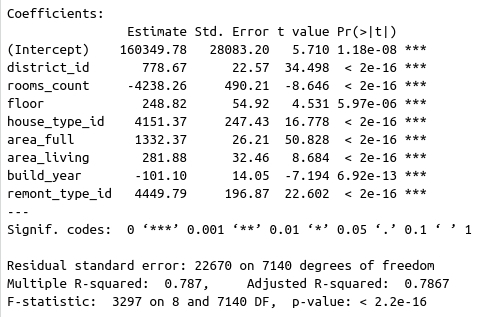
\includegraphics[scale=0.8]{multiple_model.jpg}
  \caption{Характеристики множественной модели регрессии}
  \label{fig:experiment:multiple_model}
\end{figure}

Построенные отдельно модели по числу спален показали схожие результаты и коэффициент детерминации $R^2$ равен 0.64.
Полученная матрица корреляции представлена на рисунке~\ref{fig:experiment:corr_matrix}. Исходя из данной матрицы можно 
сделать вывод что на конечную цену существенное влияние оказывает средняя цена проданной недвижимости, средняя цена аренды,
тип объекта недвижимости и площадь объекта.

\begin{figure}[!ht]
  \centering
  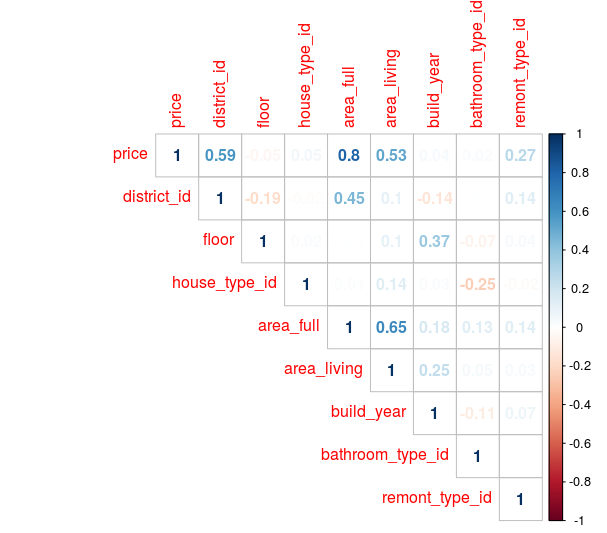
\includegraphics[scale=1]{corr_matrix.png}
  \caption{Матрица корреляции}
  \label{fig:experiment:corr_matrix}
\end{figure}

На рисунке~\ref{fig:experiment:comparing_results} приведено сравнение прогнозируемой цены на недвижимиость
с фактической. Можно видеть, что полученная модель не позволяет точно прогнозировать цену на объект недвижимости ввиду
большой погрешности. Исходя из этого можно сделать вывод, что предложенная модель оказалась неэффективной и не может быть
использована для прогнозирования цены.

\begin{figure}[!ht]
  \centering
  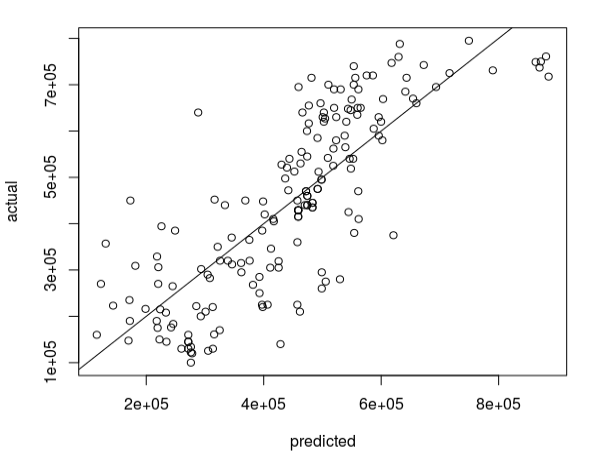
\includegraphics[scale=0.8]{comparing_results.png}
  \caption{Сравнение прогнозируемой цены с фактической}
  \label{fig:experiment:comparing_results}
\end{figure}
